%---------------------------------------------------------------------------------------------------
%		platform.tex
%
%	This file contains the sections that describe available IaaS cloud platform and its main features
%
%	Author: Andrea Meneghinello
% Version: 0.1
%	Table of changes:
%		17/03/2016 -> document definition
%---------------------------------------------------------------------------------------------------
\section{\acs{paas} cloud platforms}
\label{sec:problemSpace-cloudPlatform}
In the previous sections we have illustrated what cloud computing is and how it can make resources
available to us through the virtualization technique. 

Now we want to illustrate some of the major \ac{paas} provider competitors in the market. Each one 
has characteristics that differentiate it from the others.
Figure \ref{img:problemSpace-paas-topProviders-gartnerQuadrant} shows a snapshot of the
market (date from may 2015) of the available \ac{paas} inside a \glossarySng{gartner}. We can see
that Docker is not present and we expect that Docker company will be drawn in the chart in a future
release of Gartner chart.

In the following section we will see that some of the major competitors have started the integration
of the Docker \ac{api} inside their platforms.

\begin{figure}
	\centering{}
	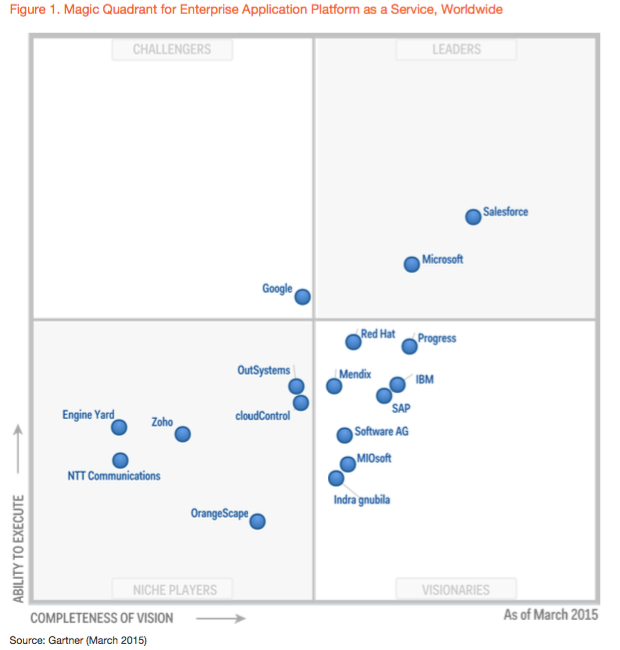
\includegraphics[width=0.8\textwidth]{chapters/problem/images/gartner-2015.png}
	\caption[Ovierviw of \acs{paas} available in 2015]{Magic Quadrant of \acf{paas}, world wide
		\cite{gartnerPaasQuadrant}.}
	\label{img:problemSpace-paas-topProviders-gartnerQuadrant}
\end{figure}

\subsection*{Google App Engine}
\label{sec:problemSpace-cloudPlatform-gae}
Google App Engine is a \ac{paas} cloud computing platform for developing and hosting web applications
in Google-managed data-centre. Applications are sandboxed and run across multiple servers. App Engine
offers automatic scaling for web applications as the number of requests increases for an application,
App Engine automatically allocates more resources for the web application to handle the additional
demand.

Google App Engine is free up to a certain level of consumed resources. Fees are charged for additional
storage, bandwidth, or instance hours required by the application.

It is offered colocated with multiple related services, including Google Compute Engine and future
Google Container Engine (both \ac{iaas}), as well as some xPaaS offerings, such as \acs{sql} and
\acs{nosql} \acs{dbms}, analytic and mobile back-end services.

Google offers it services both to small web innovators and to very large web business sites (such as
Snapchat) Additionally, Google claims that over 90\% of its internal \acs{it} is running on App Engine.

\subsection*{Microsoft Windows Azure}
\label{sec:problemSpace-cloudPlatform-azure}
Microsoft Azure is a cloud computing platform and infrastructure created by Microsoft for building, 
deploying, and managing applications and services through a global network of Microsoft-managed
data-centres.

It provides both \ac{paas} and \ac{iaas} services and supports many different programming languages,
tools and frameworks, including both Microsoft-specific and third-party software and systems.

Microsoft \ac{paas} is part of a larger Azure cloud platform, where other \ac{paas} capabilities,
including \acs{dbms}, analytics, batch and identity management, and other services, are combined with
\ac{iaas} capabilities, including compute and storage services. This cloud platform enables on-cloud
integration of older and new application software and databases.

Microsoft Azure is available in Microsoft or partner-owned data-centres in all major geographic regions.

\subsection*{Red Hat openshift}
\label{sec:problemSpace-cloudPlatform-openshift}
OpenShift is a \ac{paas} product from Red Hat. The software that runs the service is open-sourced
under the name OpenShift Origin, and is available on GitHub. Developers can use Git to deploy web 
applications in different languages on the platform. A business version for cloud computing is named
OpenShift Enterprise. It also allows the use of arbitrary languages and frameworks. OpenShift takes
care of maintaining the services underlying the applications and scaling them as needed. It supports
multiple language environments, such as .NET. Various databases and web application frameworks are also
supported.

Red Hat provides two configurations of its public \ac{paas}: OpenShift online is a shared-\acs{os}
public \ac{paas}, and OpenShift Online Dedicated Node Services is an optimized shared-hardware public
\ac{paas}, in which each tenant has exclusive use of its \ac{vm}s. Red Hat also provides OpenShift 
Enterprise, which IT organizations can use to build a private \ac{paas} environment. All variants of
OpenShift run on \ac{rhel}, and it can be deployed on \ac{aws}, OpenStack, VMware or bare metal.
OpenShift origin is available for free download without support.

OpenShift supports multiple middleware environments and languages using a plug-in cartridge model.
Cartridges are deployed into Linux containers (called Gears), which allocate system resources to
tenants and ensure tenant isolation.

In the next version of OpenShift, Red Hat will replace its Gear container \acs{api} with Docker.
Full support for Docker will produce a number of advantages: users will be able to deploy any Docker
image into an OpenShift Gear; they will have access to the huge ecosystem of Docker images on Docker
Hub; and Docker images will deploy faster than cartridge packages.

\subsection*{Docker data center}
\label{sec:problemSpace-cloudPlatform-datacentre}
At the end of February Docker announced \cite{dockerDatacentre} the release of its data-centre which
brings containers management and services deployment to the enterprise with a production ready
\ac{caas} that is supported by Docker and hosted locally, behind their firewalls.

The biggest difference between Docker data-centre and other \ac{paas} providers is that Docker \ac{caas}
is an end-to-end fully Docker-native platform. This means that users can utilize the Docker \ac{cli}
and the full set of \acs{api}. The platform is extremely pluggable as they believe in the philosophy of
``batteries included, but swappable.'' Users can simply plug Docker \ac{caas} into their existing
environments, avoiding vendor lock-in.

\ac{paas} solutions are notorious for locking customers into using a particular infrastructure. They
are often cobbled together solutions that are not natively integrated. For instance, you could use
something like OpenShift, but then your orchestration might be Kubernetes, while also using the open
source Docker engine.